%%%%%%%%%%%%%%%%%%%%%%%%%%%%%%%%%%%%%%
%%%%%%%%%%%%%%%%%%%%%%%%%%%%%%%%%%%%%%
% Do not edit the TeX file your work
% will be overwritten.  Edit the RnW
% file instead.
%%%%%%%%%%%%%%%%%%%%%%%%%%%%%%%%%%%%%%
%%%%%%%%%%%%%%%%%%%%%%%%%%%%%%%%%%%%%%





\newcommand{\DefineMacros}{
\newcommand{\AlexNSur}{4,364}
\newcommand{\AlexNTar}{4,085,282}
\newcommand{\AlexSurmean}{0.462}
\newcommand{\AlexMrp}{0.288}
\newcommand{\AlexMrpSD}{0.0169}
\newcommand{\AlexRaking}{0.263}
\newcommand{\AlexRefitTimeHours}{10}
\newcommand{\AlexMrPawTimeSecs}{16}
\newcommand{\LaxNSur}{6,341}
\newcommand{\LaxNTar}{9,694,541}
\newcommand{\LaxSurmean}{0.333}
\newcommand{\LaxMrp}{0.337}
\newcommand{\LaxMrpSD}{0.039}
\newcommand{\LaxRaking}{0.33}
\newcommand{\LaxRefitTimeHours}{11}
\newcommand{\LaxMrPawTimeSecs}{23}

}


% Define the graph lists





%%%%%%%%%%%%%%%%%%%%%%
% Plots


\newcommand{\AlexanderWeightPlot}{

\begin{knitrout}
\definecolor{shadecolor}{rgb}{0.969, 0.969, 0.969}\color{fgcolor}\begin{figure}[!h]

{\centering 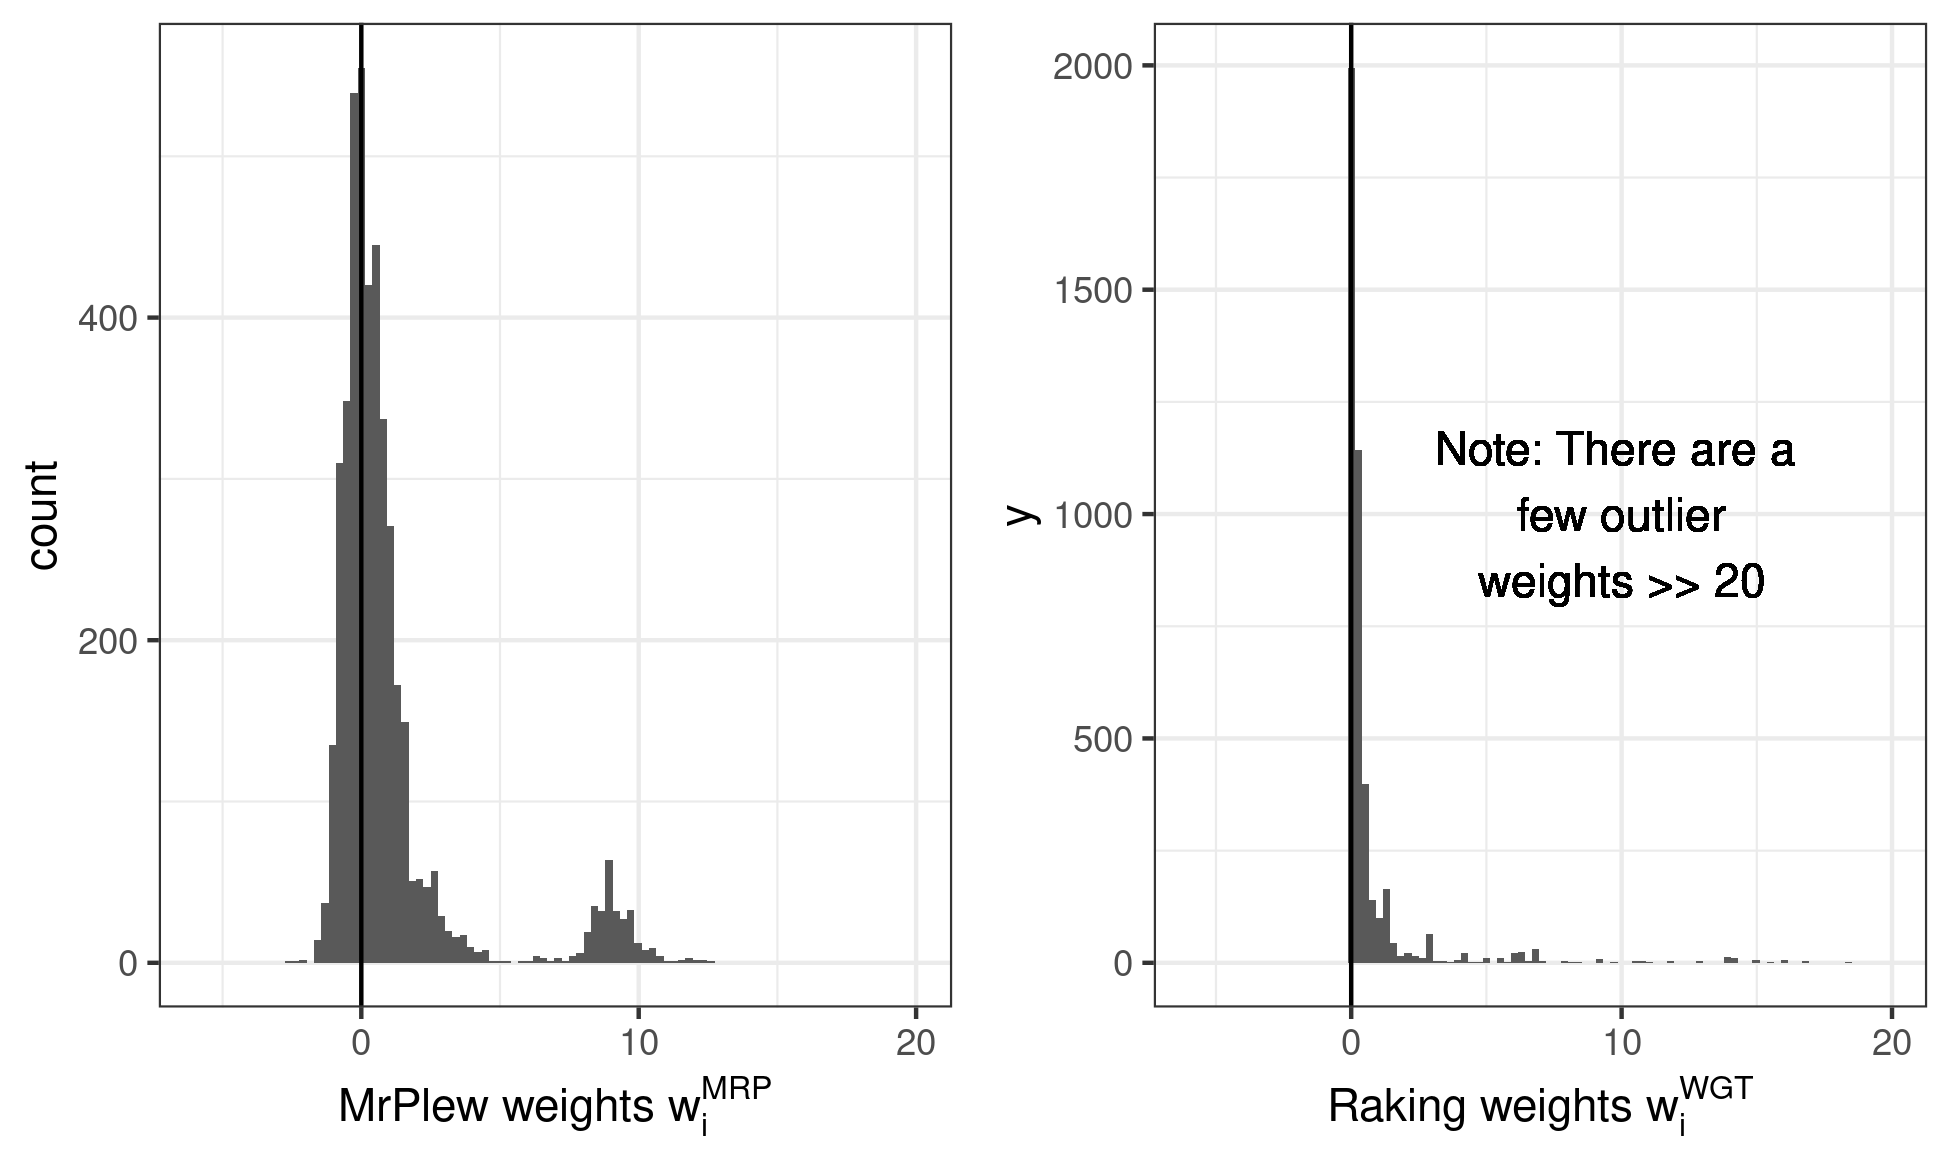
\includegraphics[width=0.98\linewidth,height=0.588\linewidth]{figure/alexanderweightplot-1} 

}

\caption[Comparison between raking and MrPlew weights for the Name Change dataset]{Comparison between raking and MrPlew weights for the Name Change dataset}\label{fig:alexanderweightplot}
\end{figure}

\end{knitrout}
}


\newcommand{\LaxWeightPlot}{

\begin{knitrout}
\definecolor{shadecolor}{rgb}{0.969, 0.969, 0.969}\color{fgcolor}\begin{figure}[!h]

{\centering 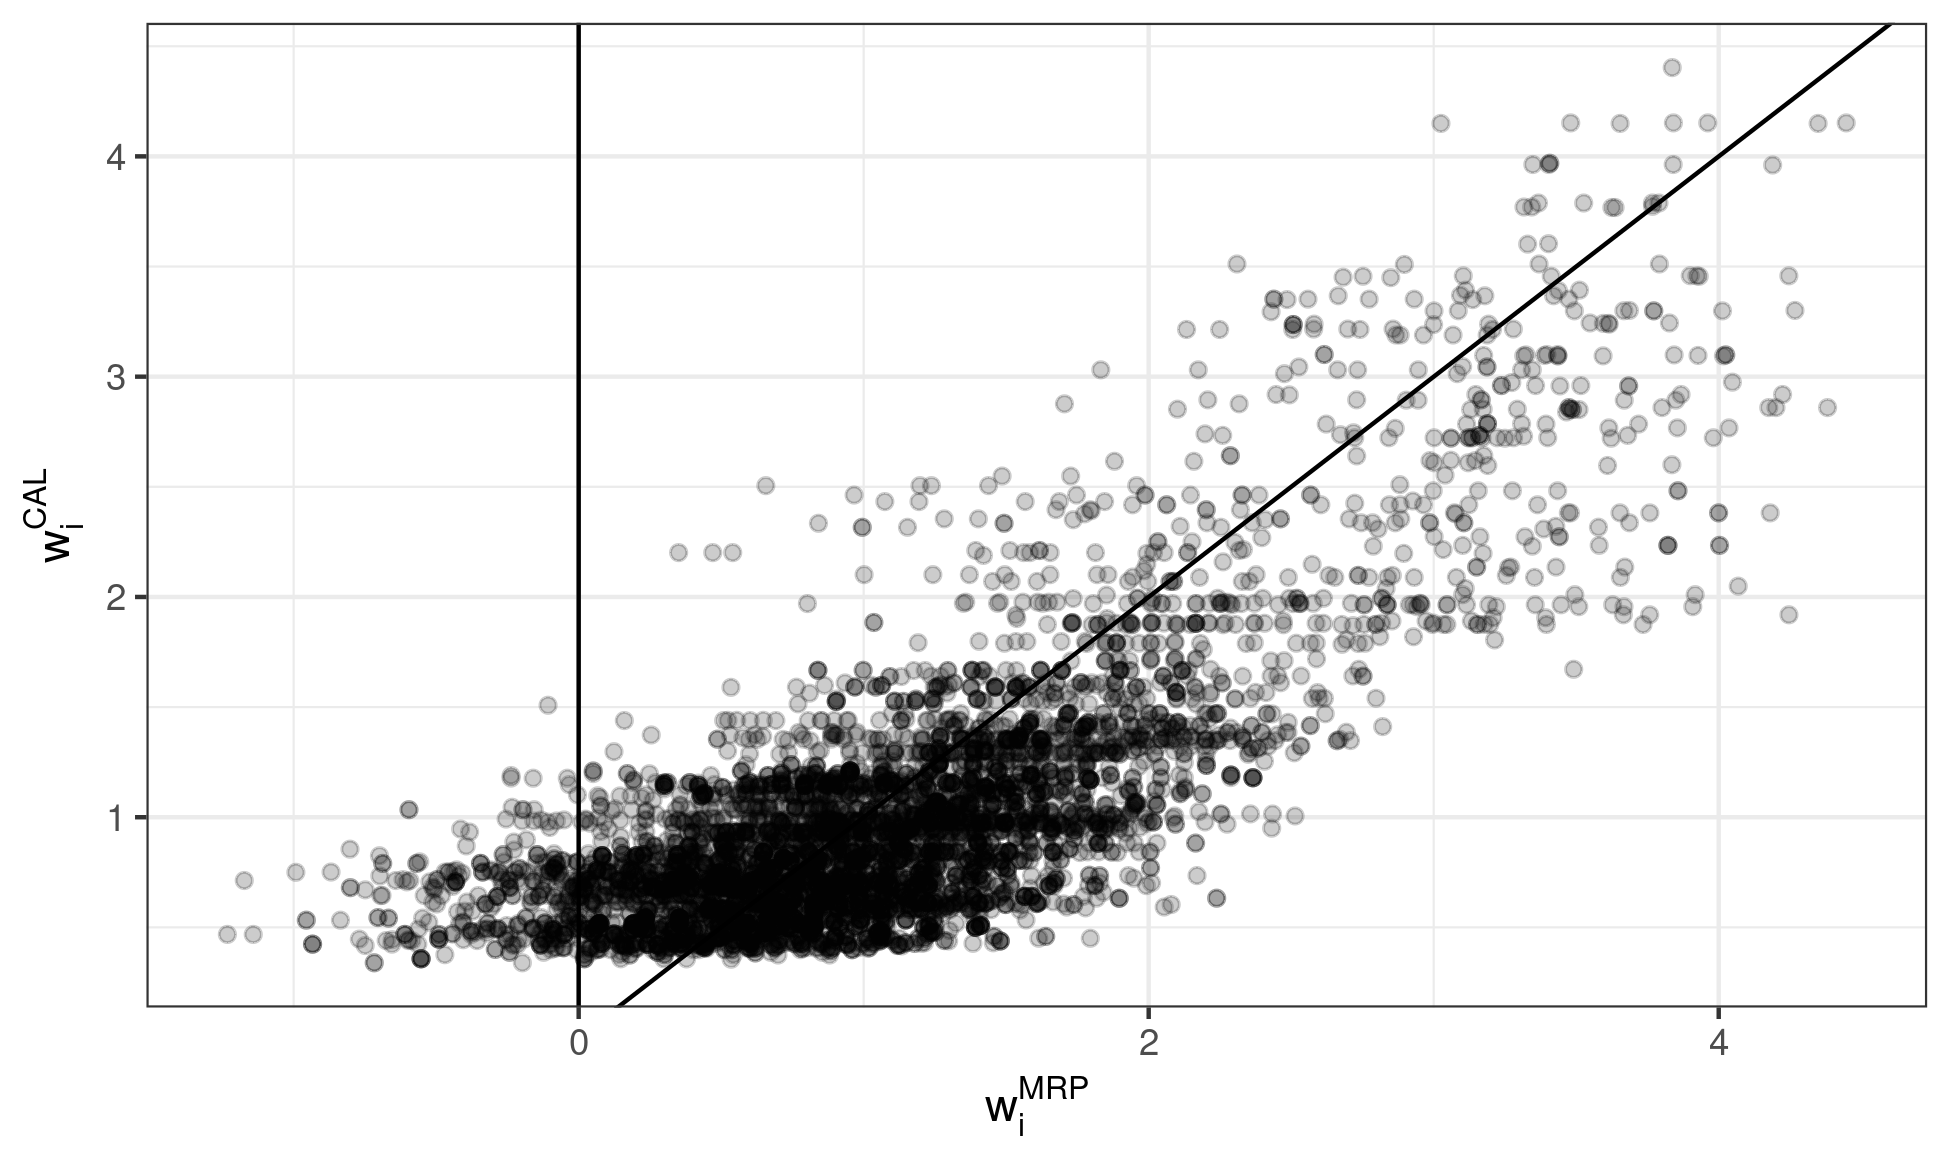
\includegraphics[width=0.98\linewidth,height=0.588\linewidth]{figure/laxweightplot-1} 

}

\caption[Comparison between raking and MrPlew weights for the Gay Marriage dataset]{Comparison between raking and MrPlew weights for the Gay Marriage dataset}\label{fig:laxweightplot}
\end{figure}

\end{knitrout}
}


\newcommand{\AlexanderImbalancePrimary}{

\begin{knitrout}
\definecolor{shadecolor}{rgb}{0.969, 0.969, 0.969}\color{fgcolor}\begin{figure}[!h]

{\centering 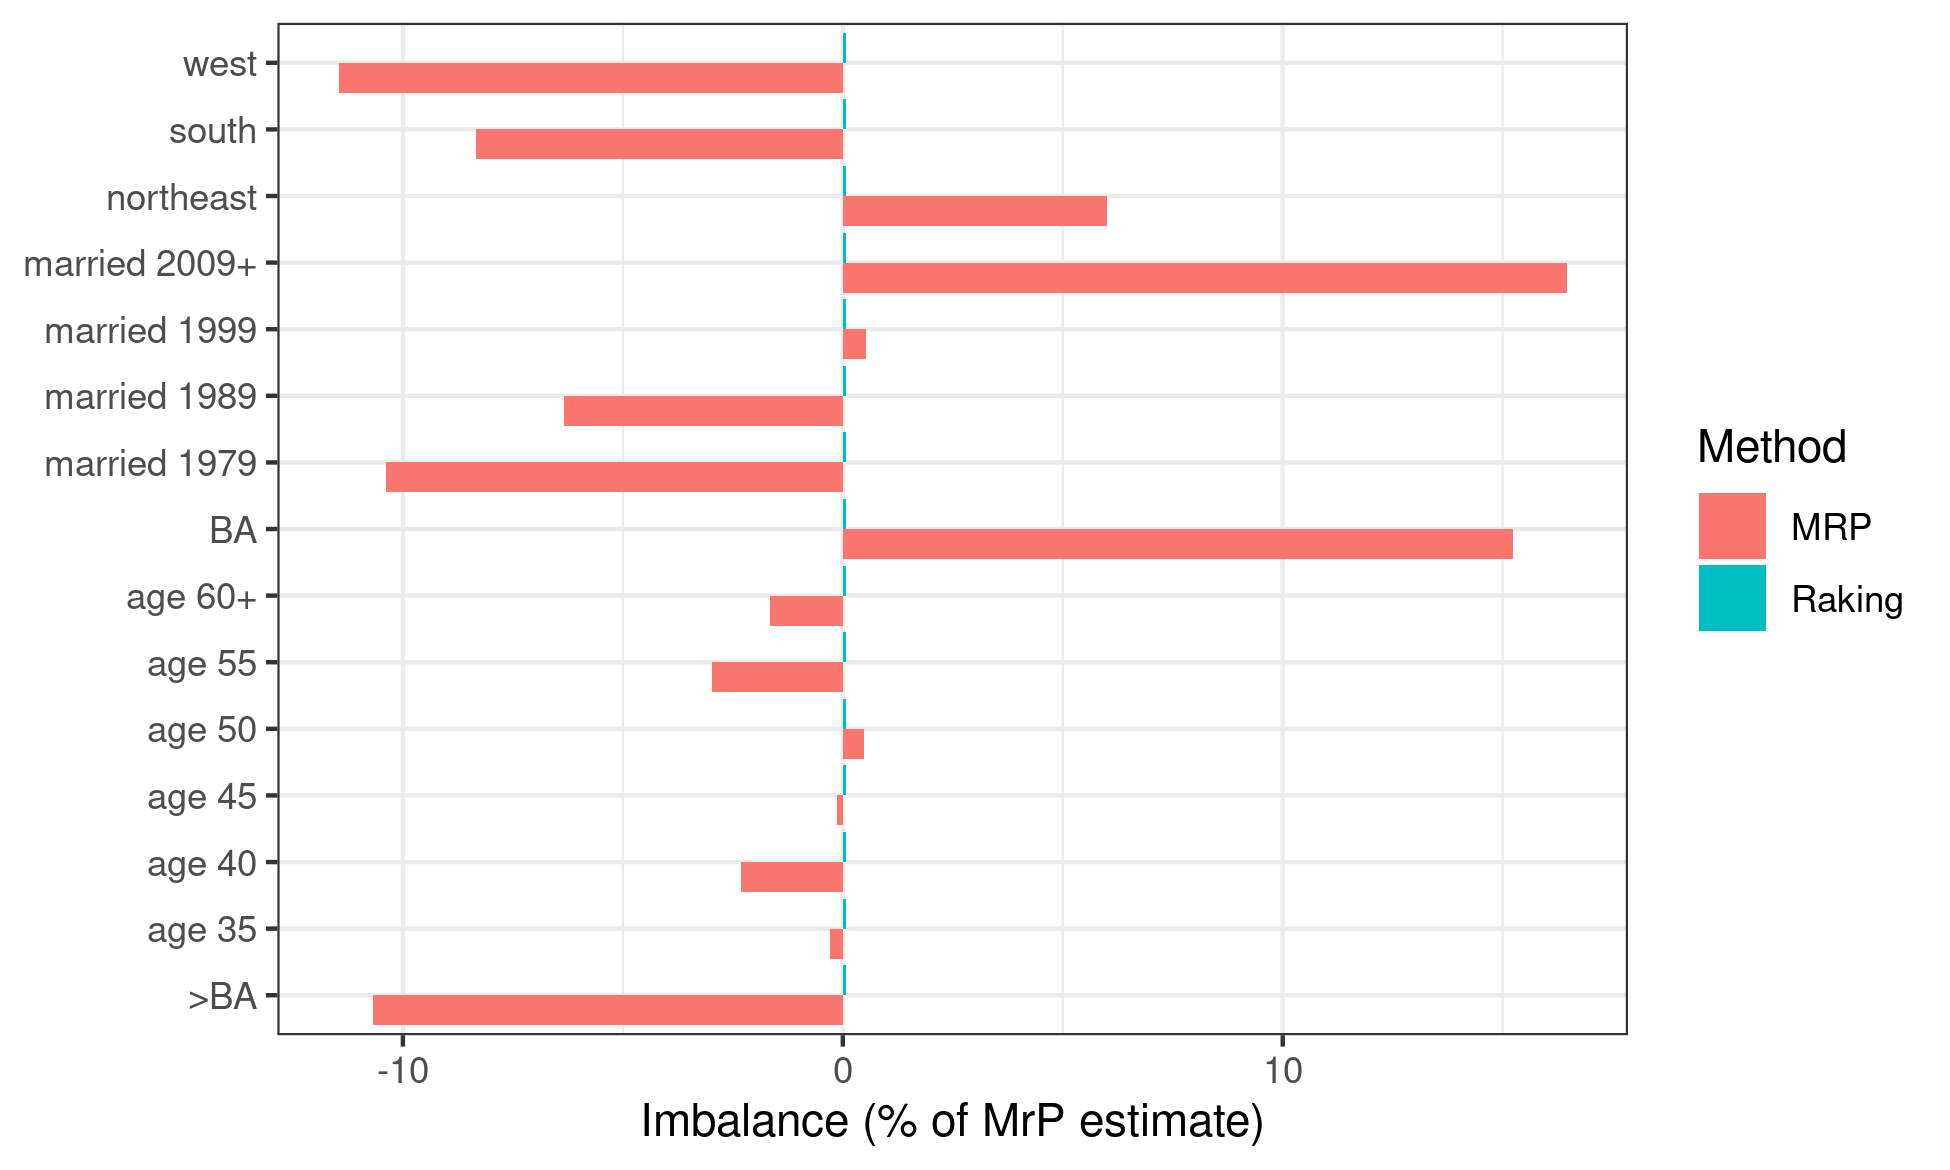
\includegraphics[width=0.98\linewidth,height=0.588\linewidth]{figure/alexanderprimary-1} 

}

\caption[Imbalance plot for primary effects in the Name Change dataset]{Imbalance plot for primary effects in the Name Change dataset}\label{fig:alexanderprimary}
\end{figure}

\end{knitrout}
}


\newcommand{\AlexanderImbalanceInteraction}{

\begin{knitrout}
\definecolor{shadecolor}{rgb}{0.969, 0.969, 0.969}\color{fgcolor}\begin{figure}[!h]

{\centering 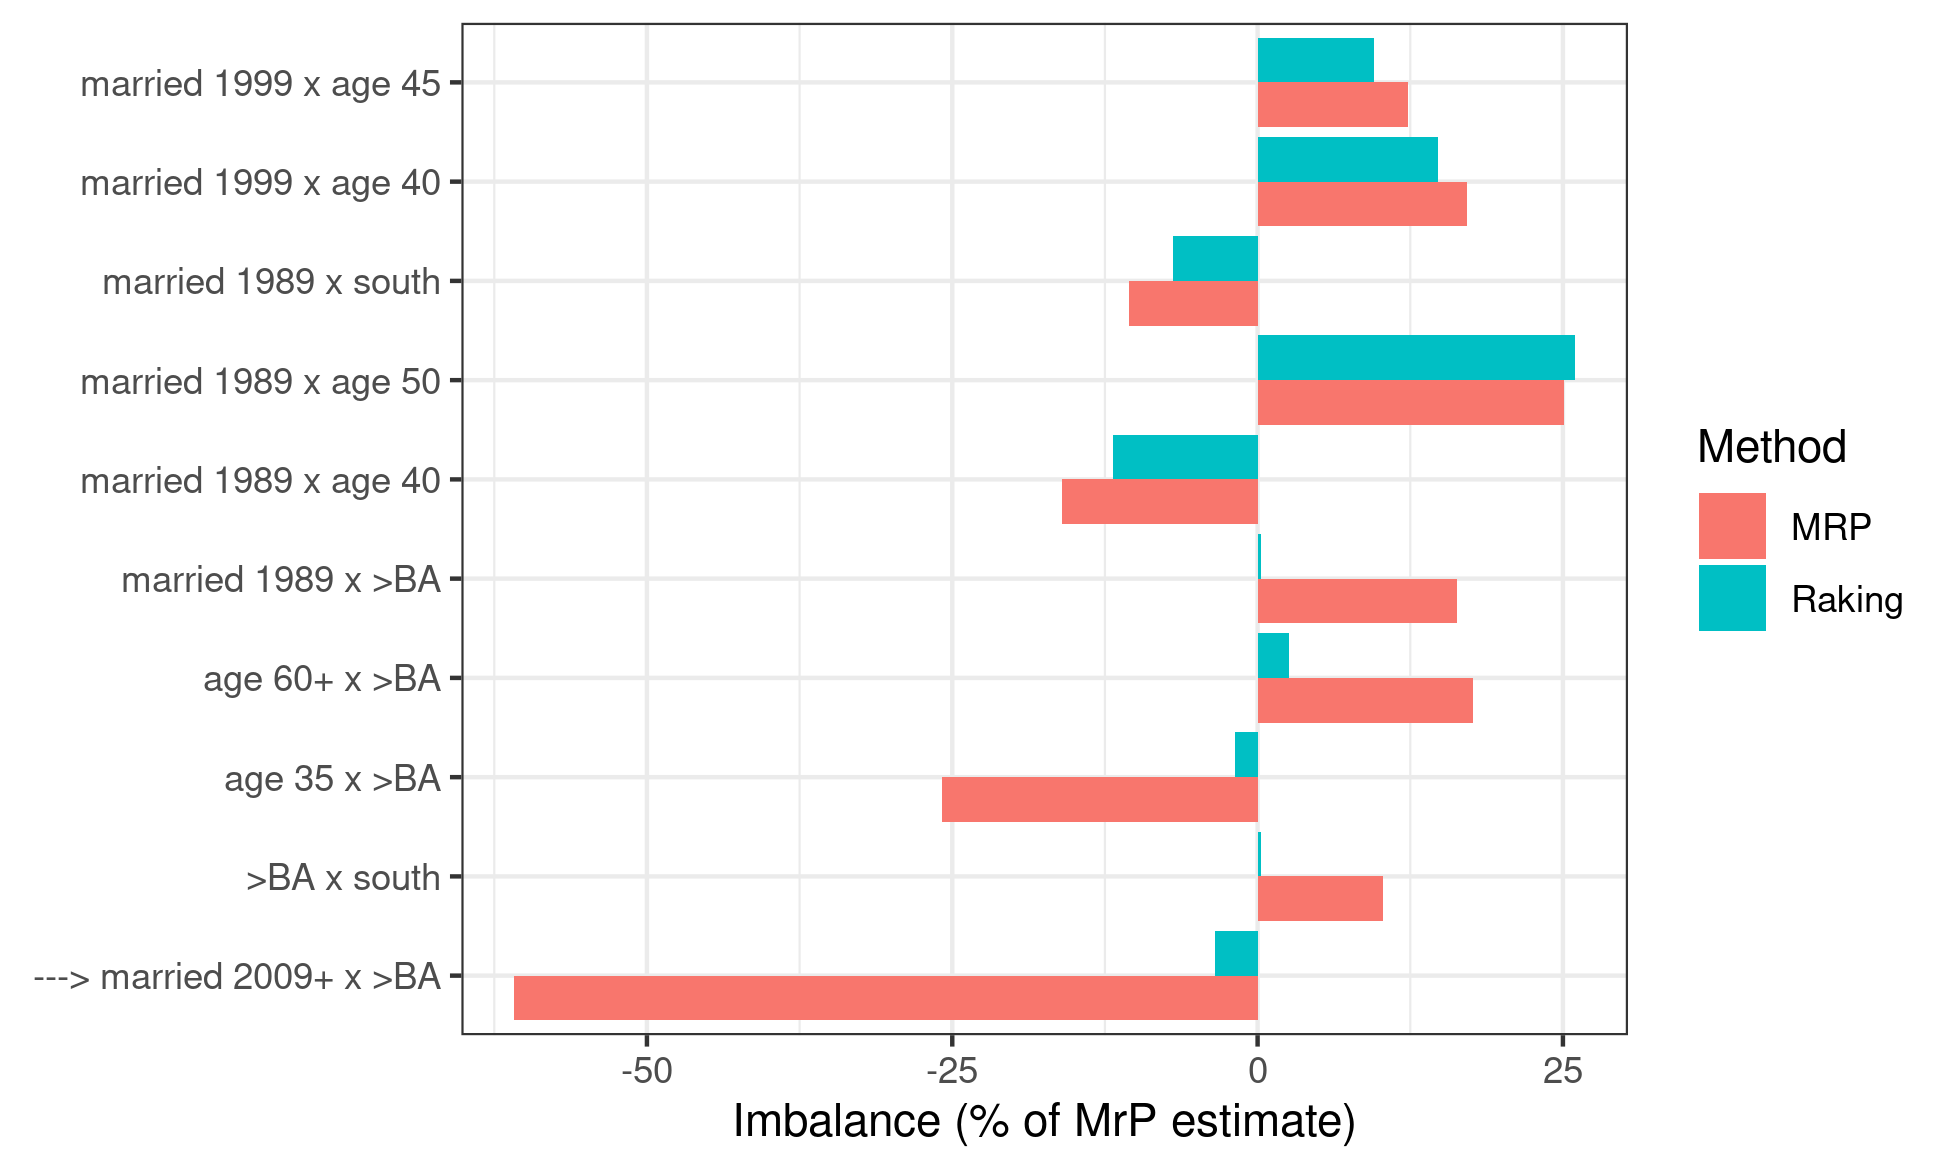
\includegraphics[width=0.98\linewidth,height=0.588\linewidth]{figure/alexanderinteraction-1} 

}

\caption[Imbalance plot for select interaction effects in the Name Change dataset]{Imbalance plot for select interaction effects in the Name Change dataset}\label{fig:alexanderinteraction}
\end{figure}

\end{knitrout}
}




\newcommand{\AlexanderPredictionFigOne}{

\begin{knitrout}
\definecolor{shadecolor}{rgb}{0.969, 0.969, 0.969}\color{fgcolor}\begin{figure}[!h]

{\centering 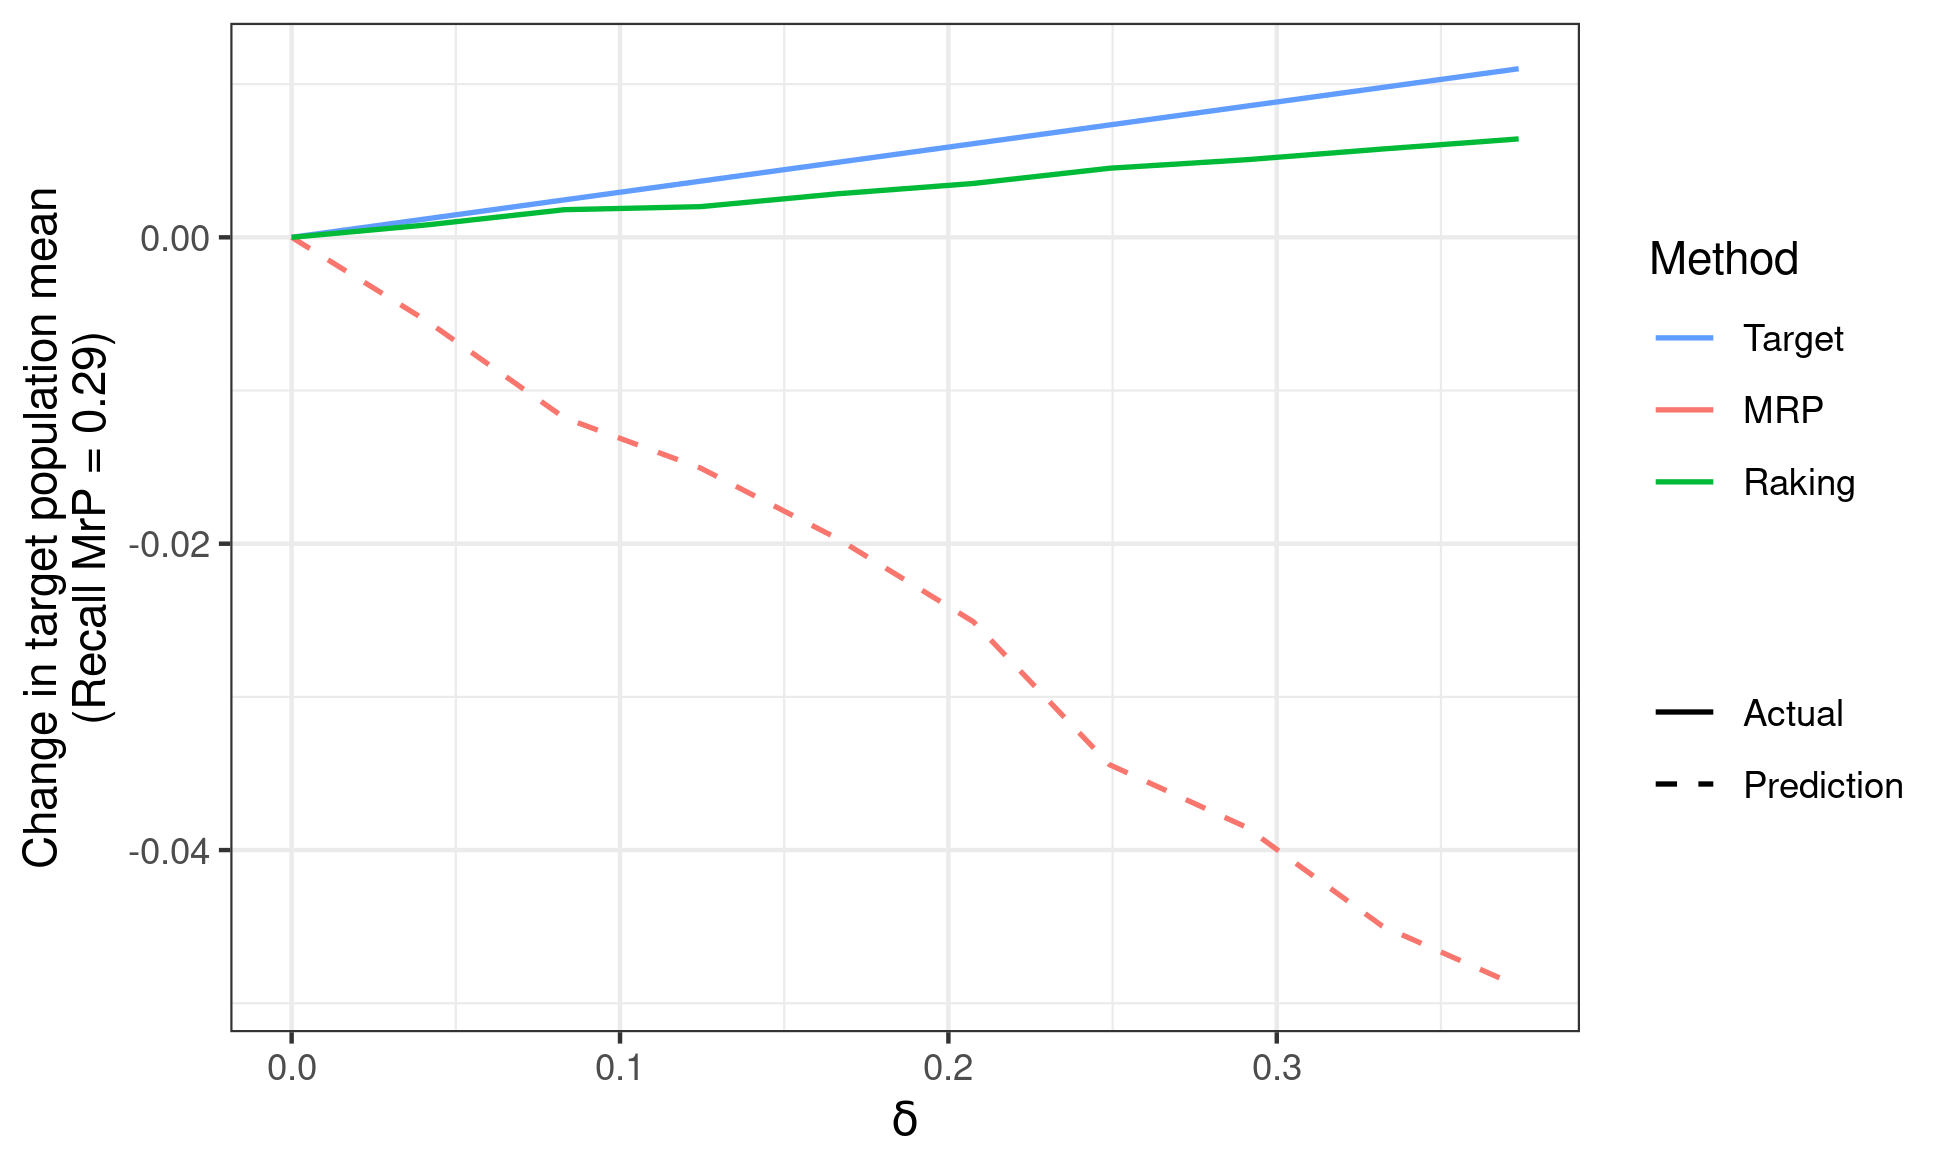
\includegraphics[width=0.98\linewidth,height=0.588\linewidth]{figure/alexandercontpred-1} 

}

\caption[Predictions on binary data for the Name Change dataset]{Predictions on binary data for the Name Change dataset}\label{fig:alexandercontpred}
\end{figure}

\end{knitrout}
}



\newcommand{\AlexanderPredictionFigTwo}{

\begin{knitrout}
\definecolor{shadecolor}{rgb}{0.969, 0.969, 0.969}\color{fgcolor}\begin{figure}[!h]

{\centering 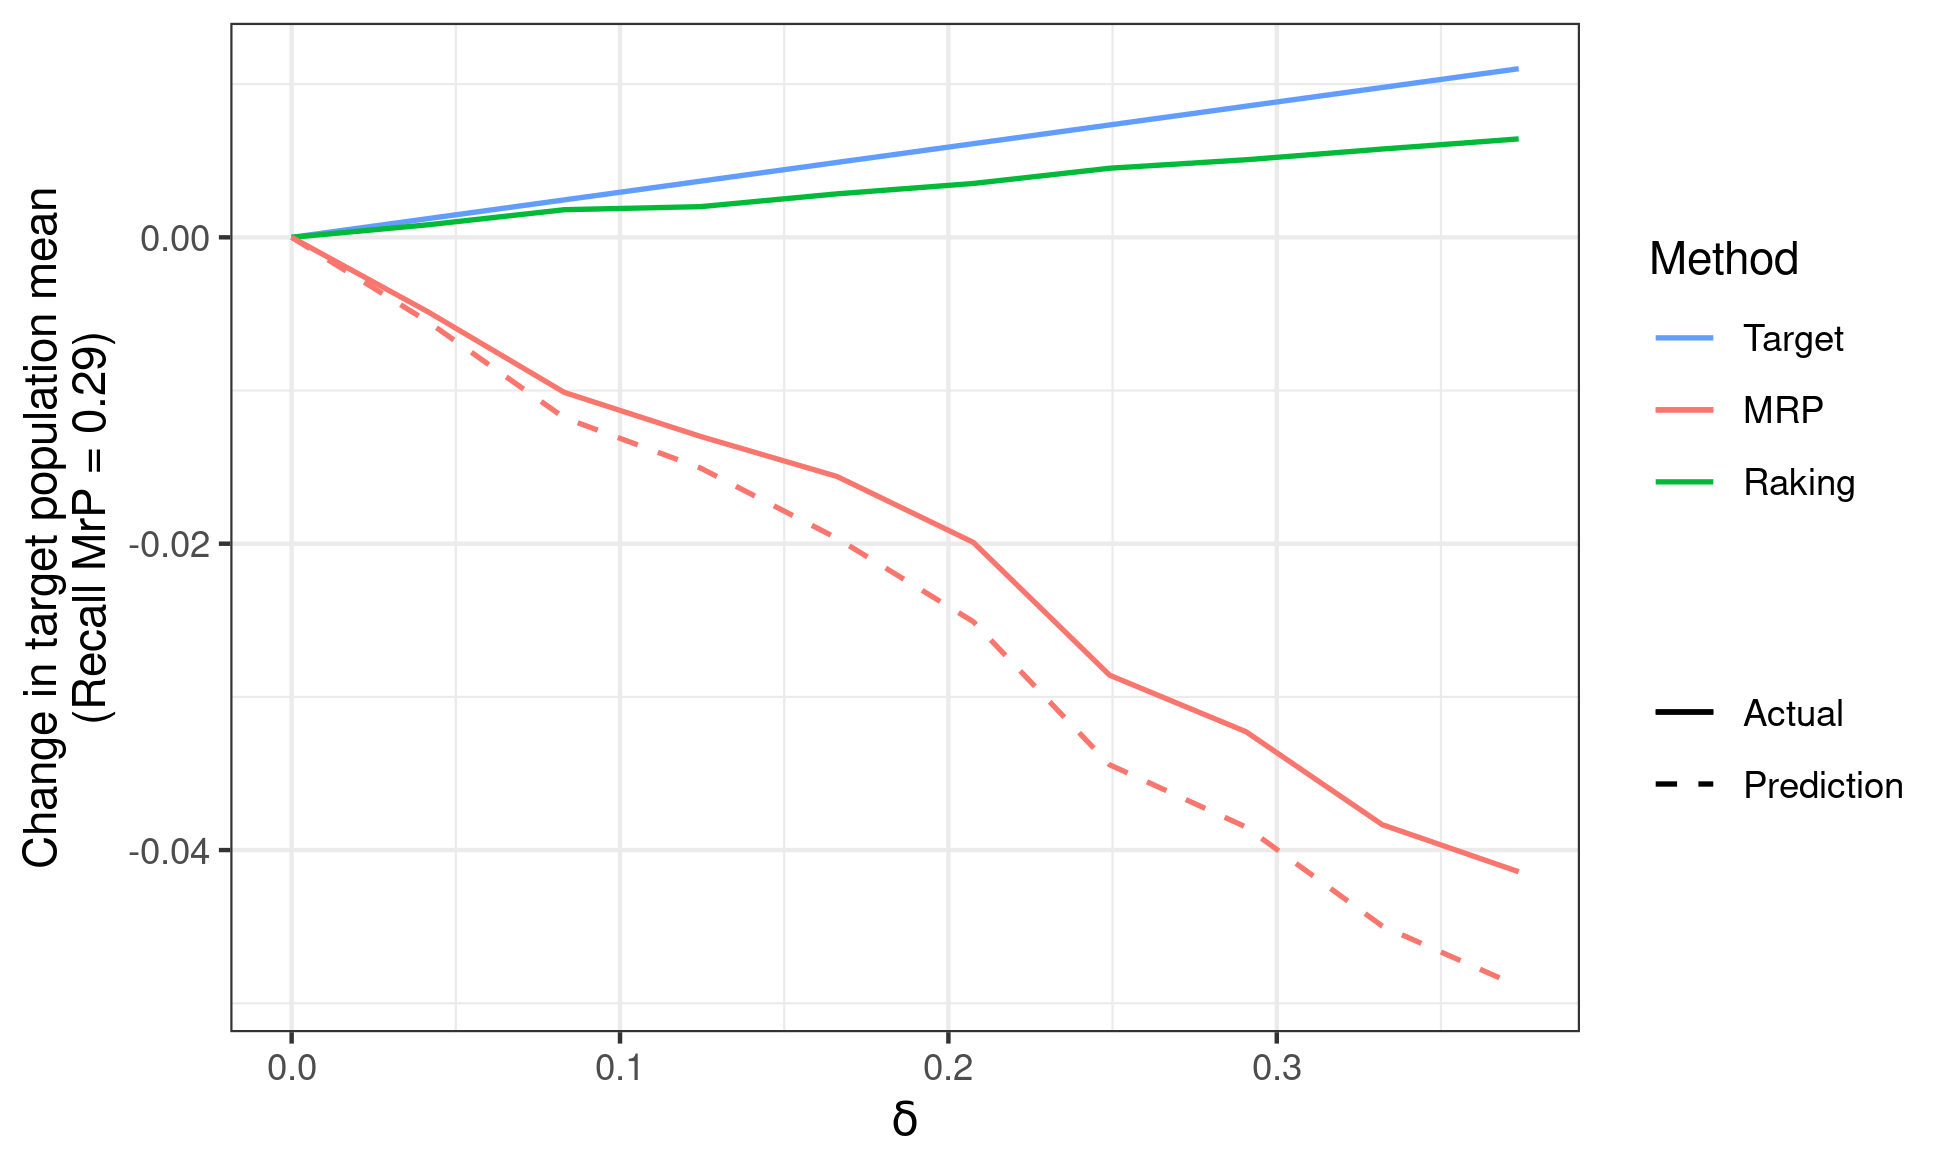
\includegraphics[width=0.98\linewidth,height=0.588\linewidth]{figure/alexanderdiscretepred-1} 

}

\caption[Predictions and refit on binary data for the Name Change dataset]{Predictions and refit on binary data for the Name Change dataset}\label{fig:alexanderdiscretepred}
\end{figure}

\end{knitrout}
}



%%%%%%%%%%%%%%%%%%%%%%



\newcommand{\LaxImbalancePrimary}{

\begin{knitrout}
\definecolor{shadecolor}{rgb}{0.969, 0.969, 0.969}\color{fgcolor}\begin{figure}[!h]

{\centering 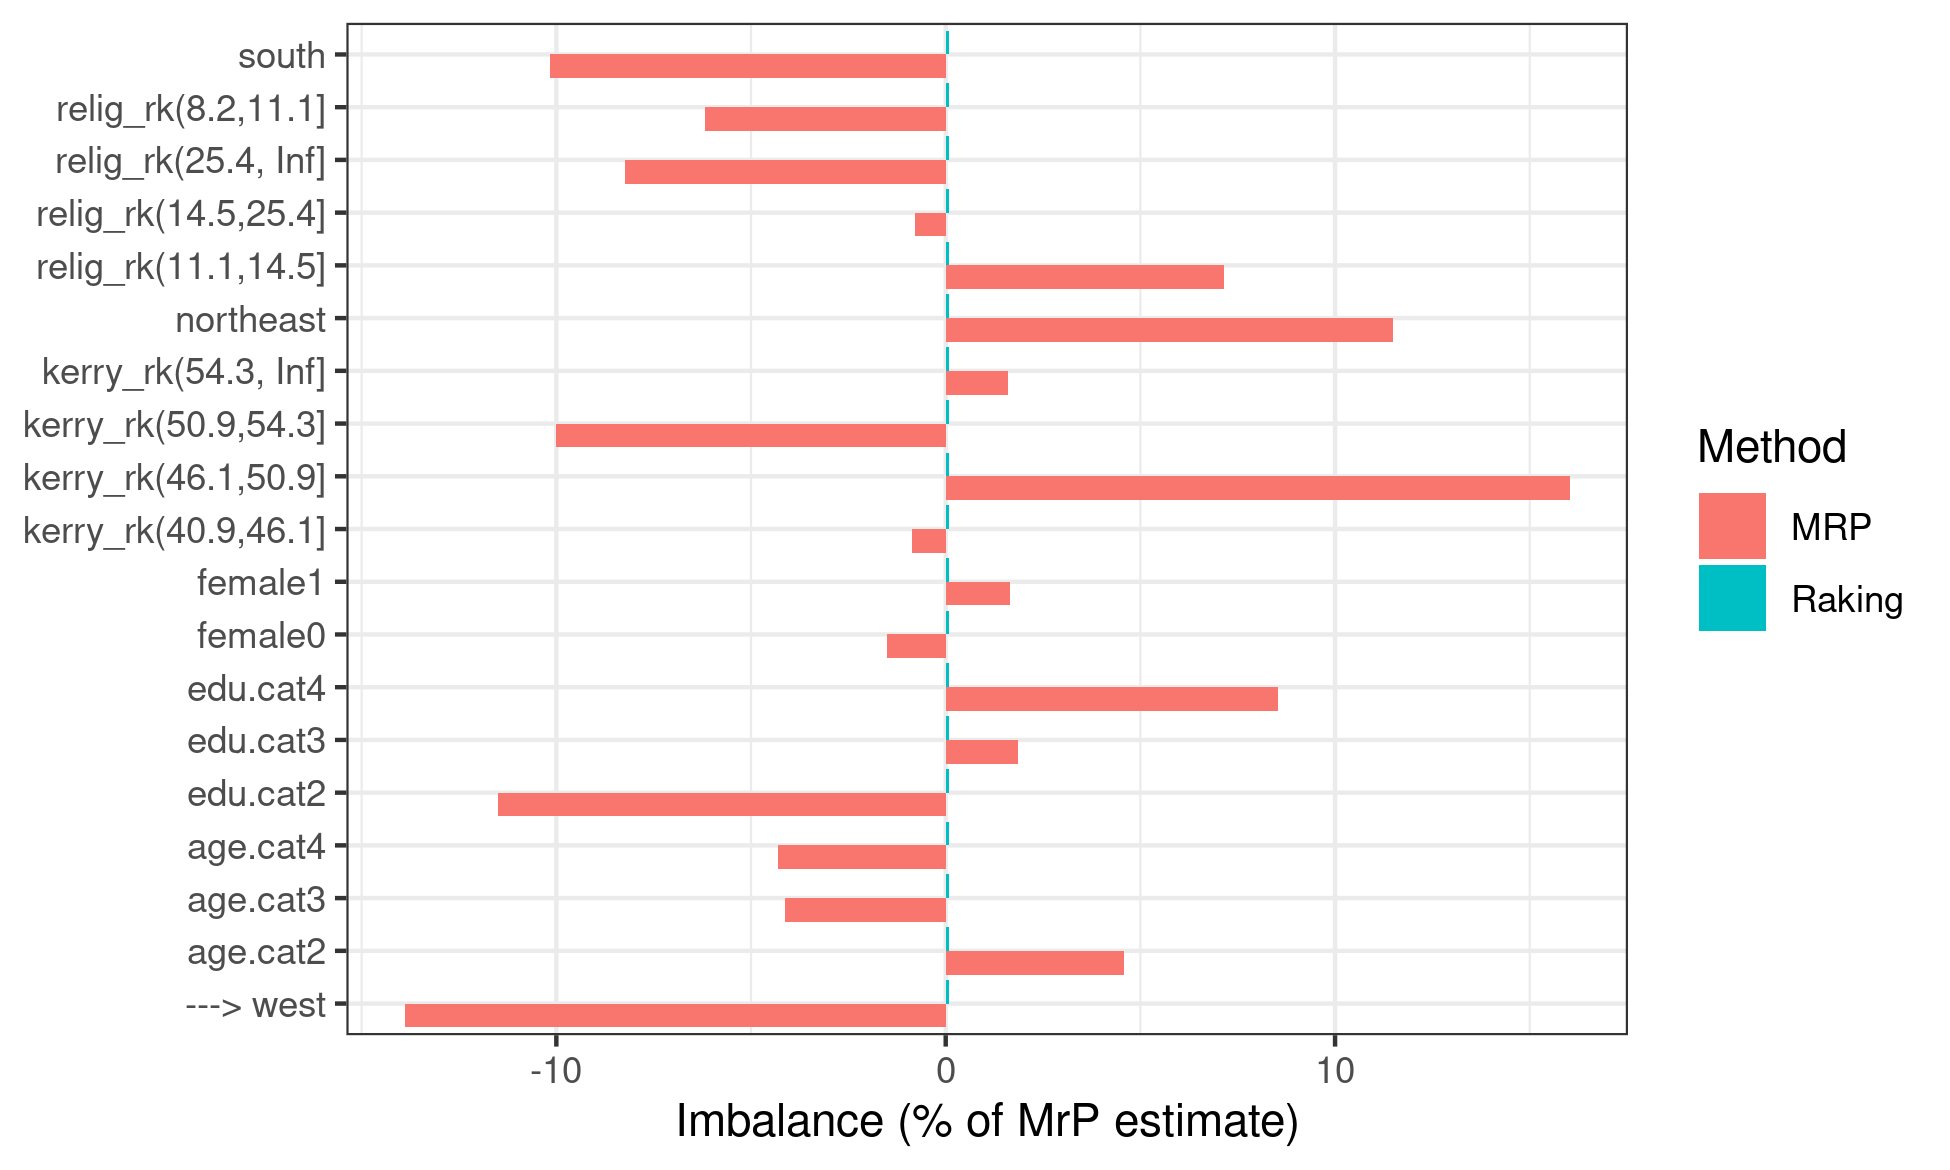
\includegraphics[width=0.98\linewidth,height=0.588\linewidth]{figure/laxprimary-1} 

}

\caption[Imbalance plot for primary effects in the Gay Marriage dataset]{Imbalance plot for primary effects in the Gay Marriage dataset}\label{fig:laxprimary}
\end{figure}

\end{knitrout}
}


\newcommand{\LaxImbalanceInteraction}{

\begin{knitrout}
\definecolor{shadecolor}{rgb}{0.969, 0.969, 0.969}\color{fgcolor}\begin{figure}[!h]

{\centering 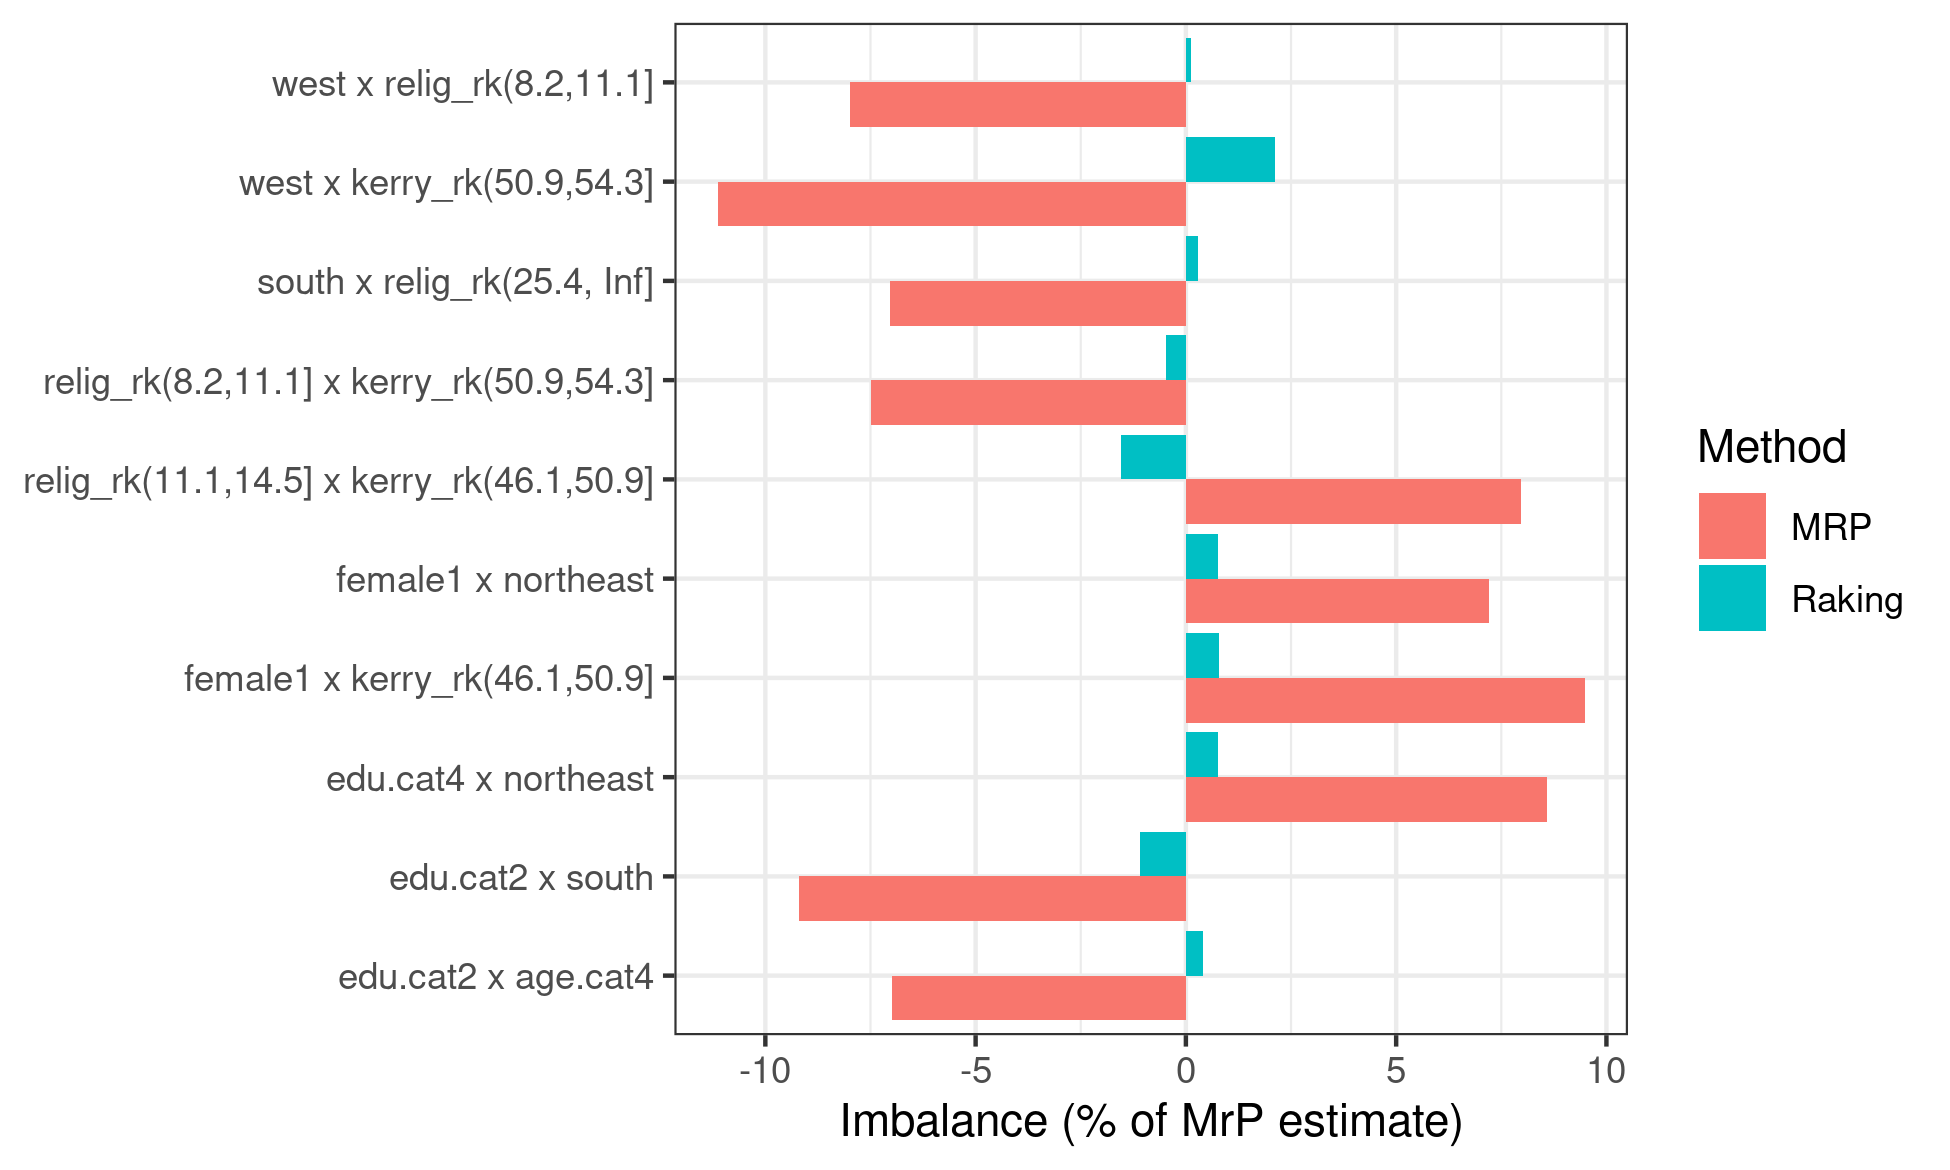
\includegraphics[width=0.98\linewidth,height=0.588\linewidth]{figure/laxinteraction-1} 

}

\caption[Imbalance plot for select interaction effects in the Gay Marriage dataset]{Imbalance plot for select interaction effects in the Gay Marriage dataset}\label{fig:laxinteraction}
\end{figure}

\end{knitrout}
}




\newcommand{\LaxPredictionFigOne}{

\begin{knitrout}
\definecolor{shadecolor}{rgb}{0.969, 0.969, 0.969}\color{fgcolor}\begin{figure}[!h]

{\centering 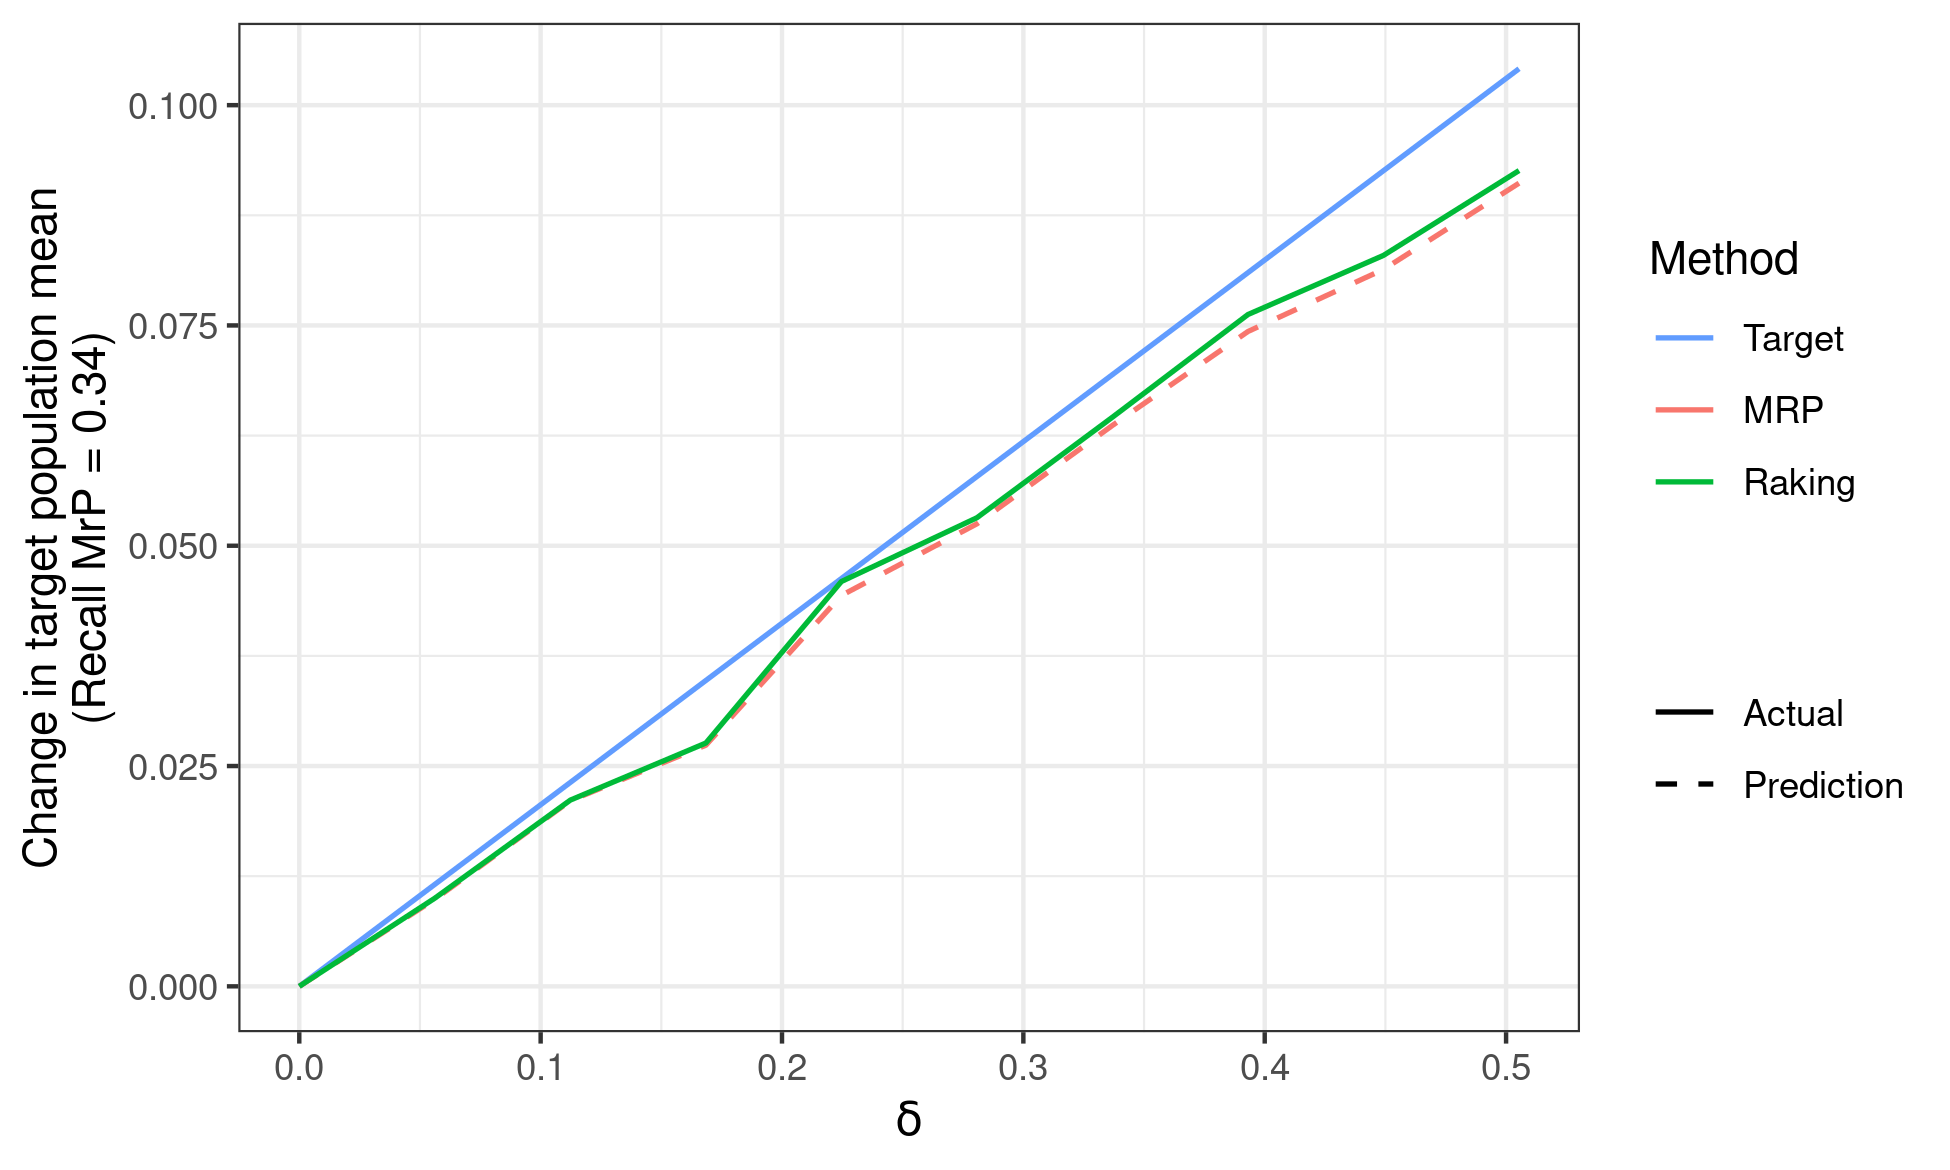
\includegraphics[width=0.98\linewidth,height=0.588\linewidth]{figure/laxcontpred-1} 

}

\caption[Predictions on binary data for the Gay Marriage dataset]{Predictions on binary data for the Gay Marriage dataset}\label{fig:laxcontpred}
\end{figure}

\end{knitrout}
}



\newcommand{\LaxPredictionFigTwo}{

\begin{knitrout}
\definecolor{shadecolor}{rgb}{0.969, 0.969, 0.969}\color{fgcolor}\begin{figure}[!h]

{\centering 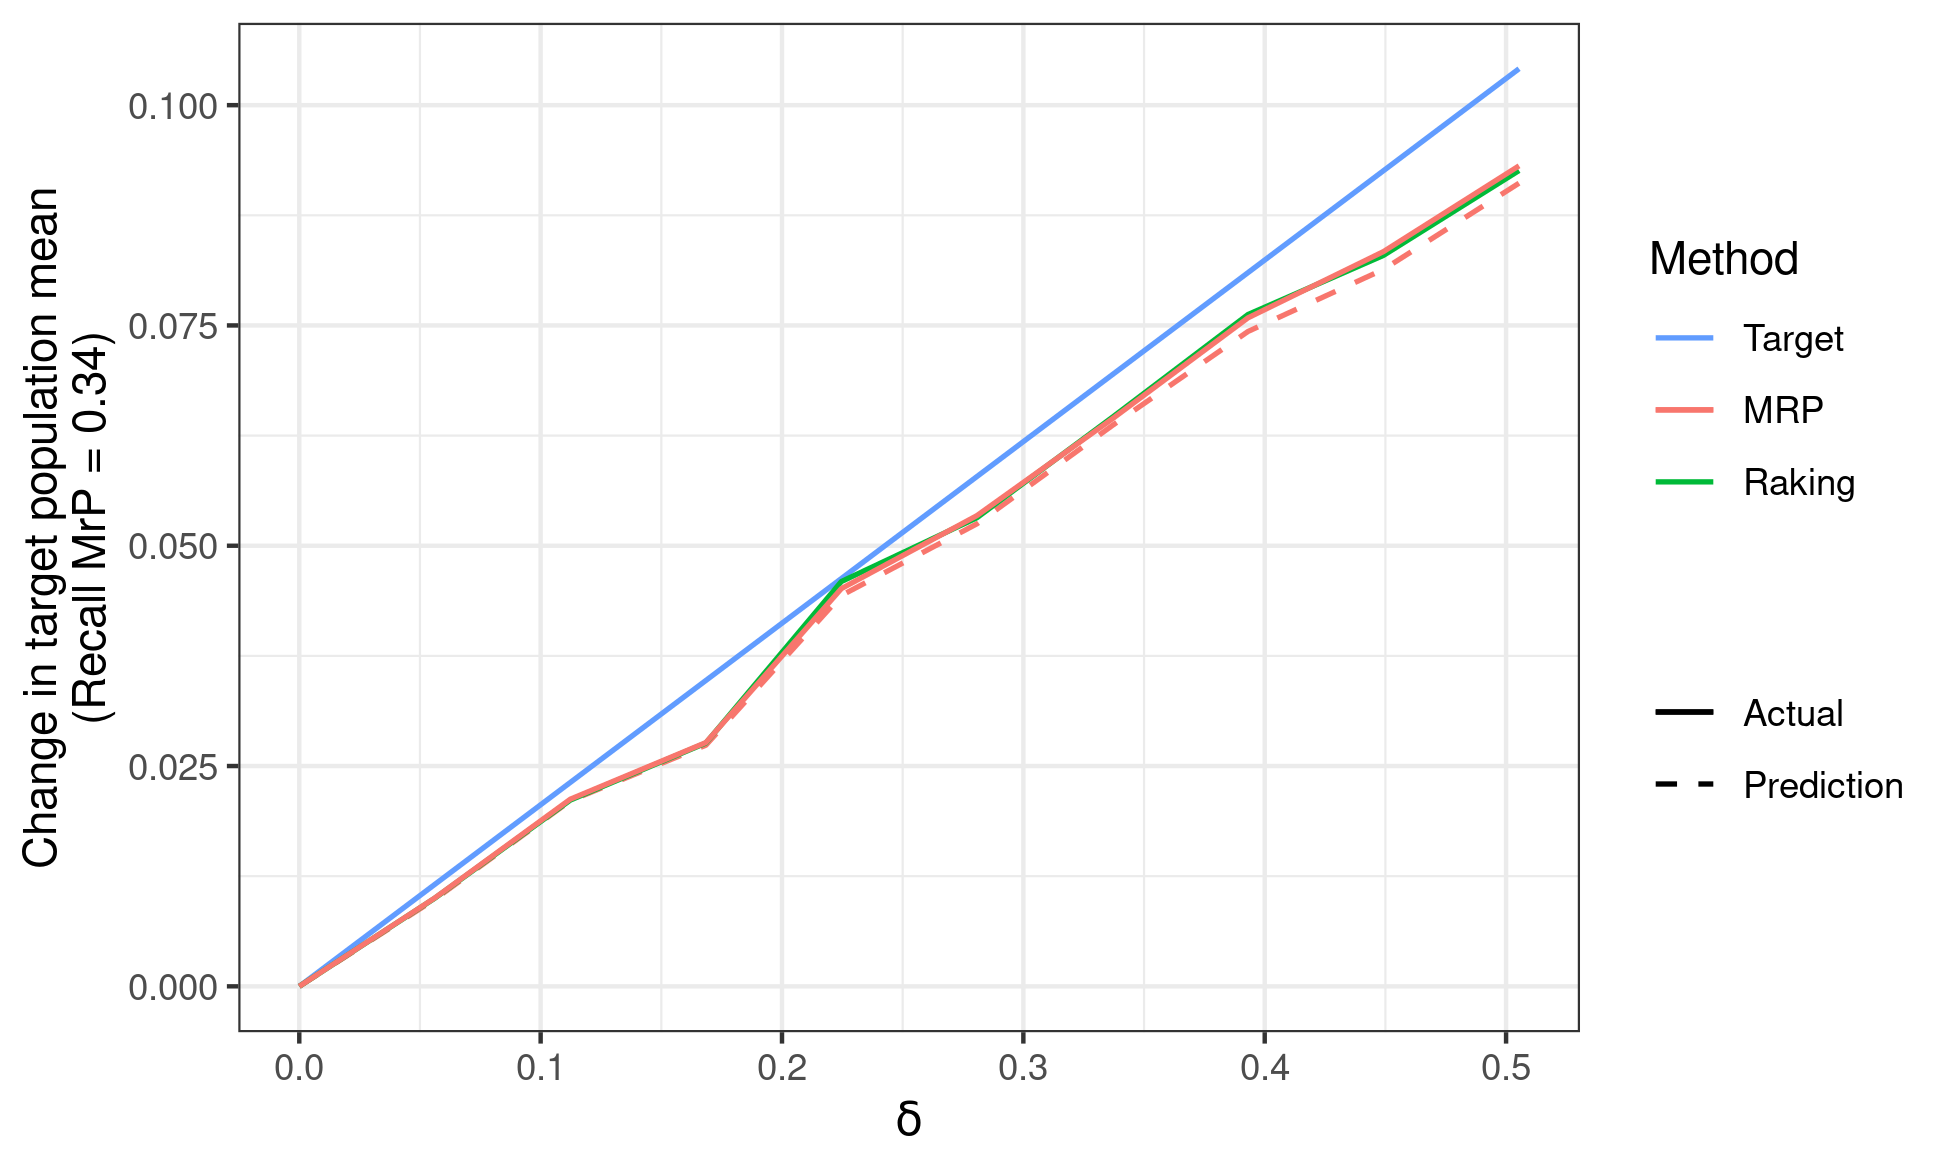
\includegraphics[width=0.98\linewidth,height=0.588\linewidth]{figure/laxdiscretepred-1} 

}

\caption[Predictions and refit on binary data for the Gay Marriage dataset]{Predictions and refit on binary data for the Gay Marriage dataset}\label{fig:laxdiscretepred}
\end{figure}

\end{knitrout}
}


%%%%%%%%%%%%%%%%%%%%%%



\newcommand{\BootstrapPlot}{

\begin{knitrout}
\definecolor{shadecolor}{rgb}{0.969, 0.969, 0.969}\color{fgcolor}\begin{figure}[!h]

{\centering 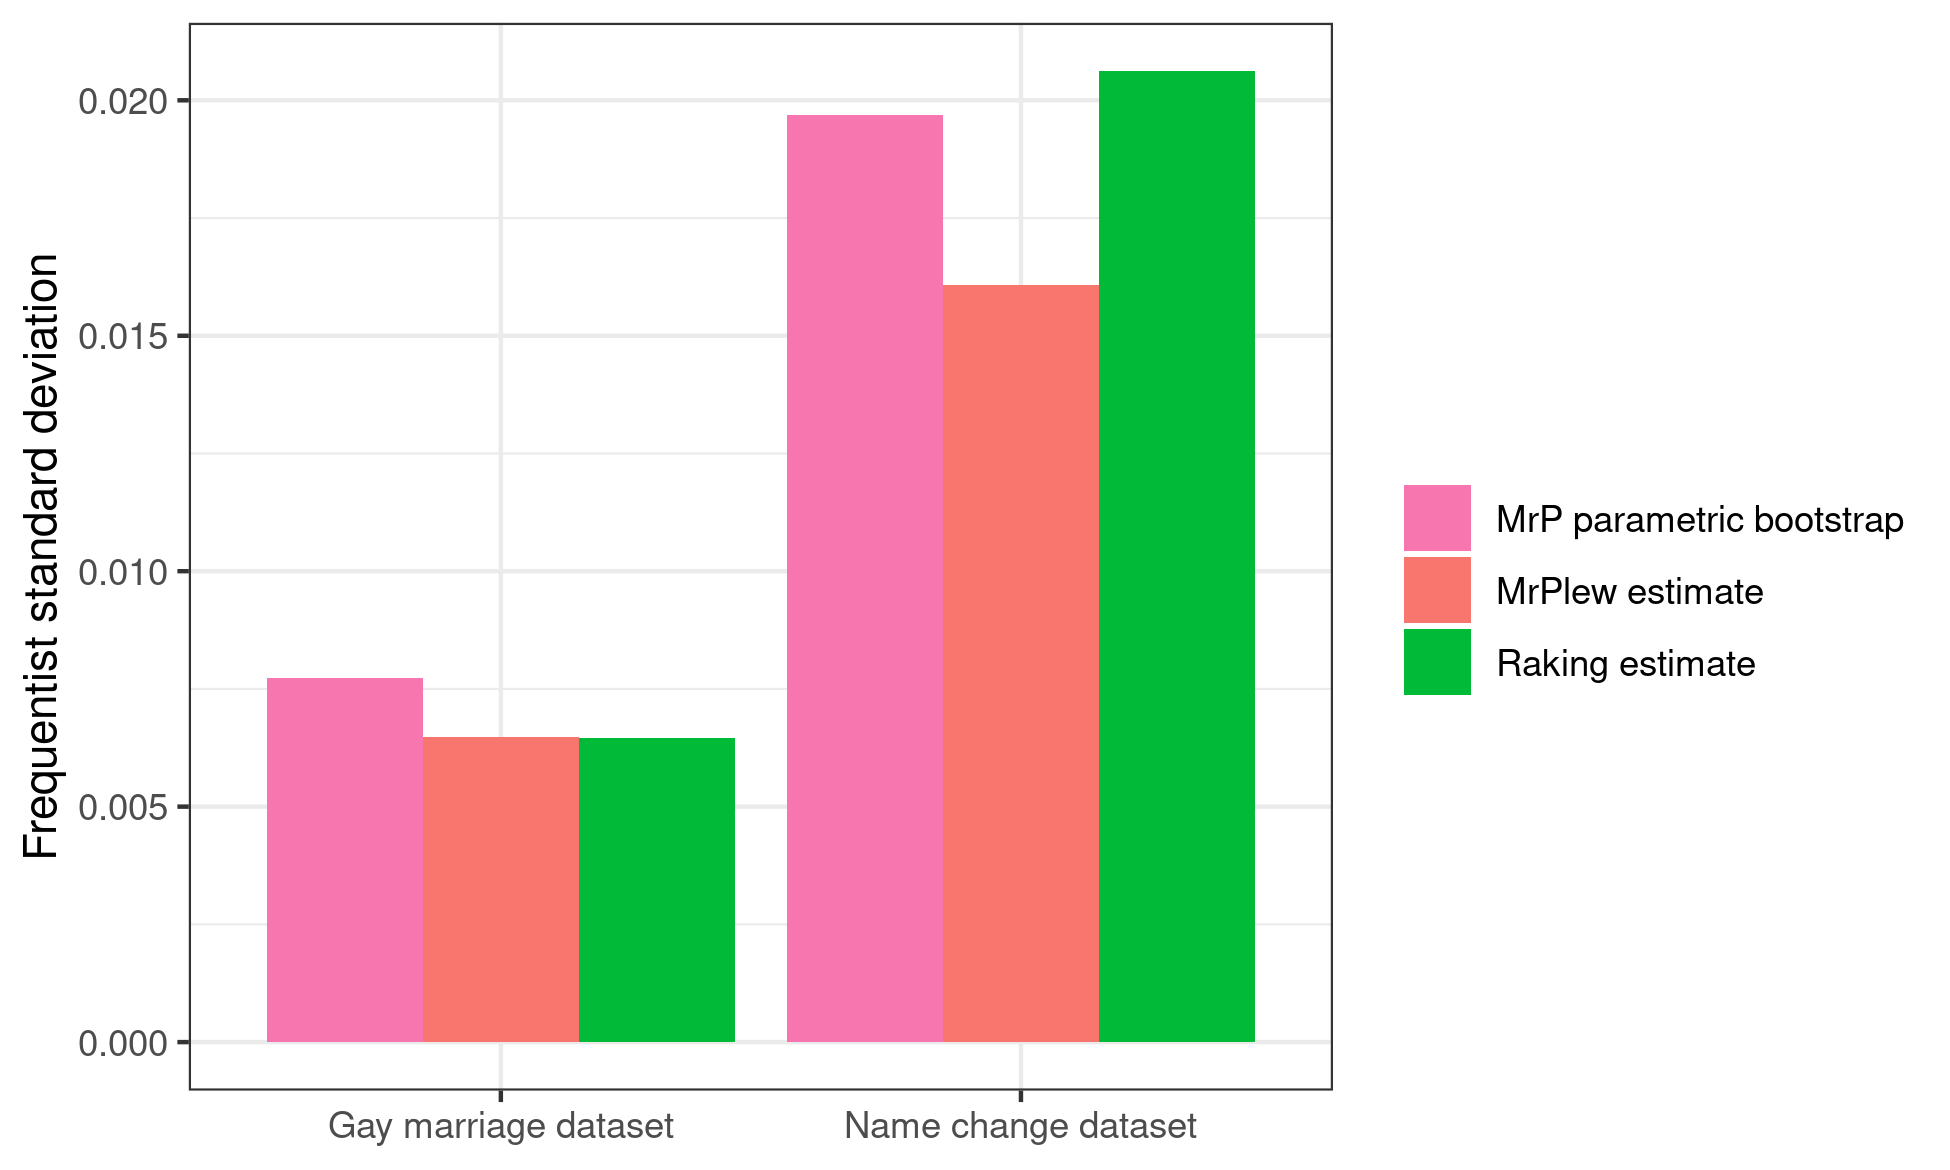
\includegraphics[width=0.98\linewidth,height=0.588\linewidth]{figure/bootplot-1} 

}

\caption[Frequentist standard deviation estimates]{Frequentist standard deviation estimates}\label{fig:bootplot}
\end{figure}

\end{knitrout}
}


%%%%%%%%%%%%%%%%%%%%%%



\newcommand{\SimulationPlot}{

\begin{knitrout}
\definecolor{shadecolor}{rgb}{0.969, 0.969, 0.969}\color{fgcolor}\begin{figure}[!h]

{\centering 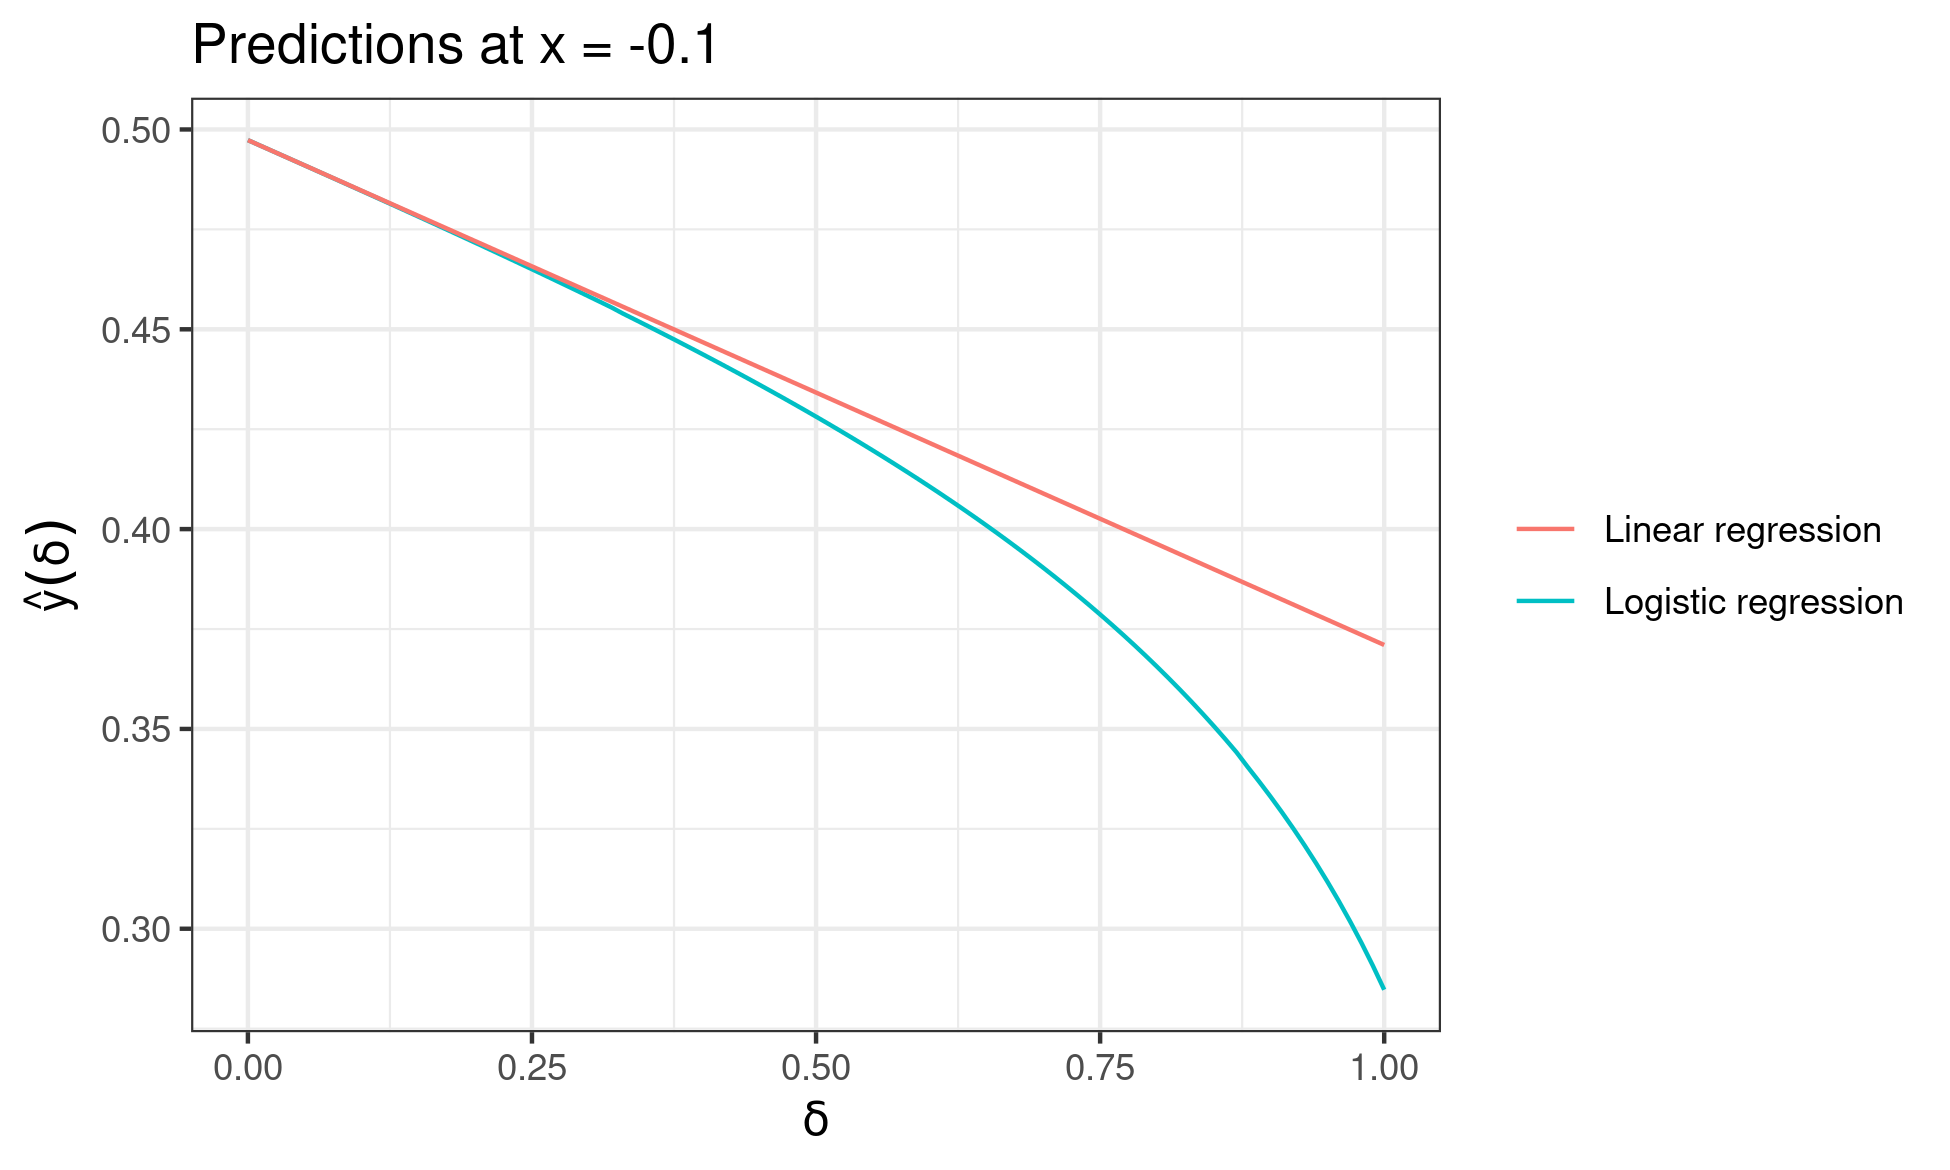
\includegraphics[width=0.98\linewidth,height=0.588\linewidth]{figure/simplot-1} 

}

\caption[Simulated path through the space of responses]{Simulated path through the space of responses}\label{fig:simplot}
\end{figure}

\end{knitrout}
}
